\documentclass[english,t]{beamer}
%\documentclass[finnish,english,handout]{beamer}

% Uncomment if want to show notes
% \setbeameroption{show notes}

\mode<presentation>
{
	\usetheme{Warsaw}
	% oder ...
	
	\setbeamercovered{invisible}
	% oder auch nicht
}

% ==============================
%  Added Package
% ==============================
\usepackage[linesnumbered,lined,commentsnumbered]{algorithm2e}
\usepackage{bm}

% =======================================
%   Using symbols for a checklist
% =======================================
\usepackage{pifont}% http://ctan.org/pkg/pifont
\newcommand{\cmark}{\ding{51}}%
\newcommand{\xmark}{\ding{55}}%

% ======================================
%     No Figure in the caption
% ======================================
\setbeamertemplate{caption}{\insertcaption} %---> does not work
%\captionsetup{labelformat=empty,labelsep=none} % ---> it works

% ===================================================
\usepackage{graphicx}
\graphicspath{{./figs/}}
\usepackage[T1]{fontenc}
\usepackage[latin1]{inputenc}
\usepackage{times}
\usepackage{epic,epsfig}
\usepackage{subfigure,float}
\usepackage{amsmath,amsfonts,amssymb}
\usepackage{inputenc}
\usepackage{babel}
\usepackage{afterpage}
\usepackage{eufrak}
\usepackage{amsbsy}
\usepackage{eucal}
\usepackage{rotating}
\usepackage{url}
\urlstyle{same}

\usepackage{natbib}
\bibliographystyle{apalike}

% \definecolor{hutblue}{rgb}{0,0.2549,0.6784}
% \definecolor{midnightblue}{rgb}{0.0977,0.0977,0.4375}
% \definecolor{hutsilver}{rgb}{0.4863,0.4784,0.4784}
% \definecolor{lightgray}{rgb}{0.95,0.95,0.95}
% \definecolor{section}{rgb}{0,0.2549,0.6784}
% \definecolor{list1}{rgb}{0,0.2549,0.6784}
\definecolor{navyblue}{rgb}{0,0,0.5}
\renewcommand{\emph}[1]{\textcolor{navyblue}{#1}}

% ===============
%    My tilde
% ===============
\newcommand{\mytilde}{\raise.17ex\hbox{$\scriptstyle\mathtt{\sim}$}}


% \graphicspath{./pics}

\pdfinfo{            
	/Title      (Bayesian data analysis 2) 
	/Author     (Aki Vehtari) % 
	/Keywords   (Bayesian probability theory, Bayesian inference, Bayesian data analysis)
}


\parindent=0pt
\parskip=8pt
\tolerance=9000
\abovedisplayshortskip=0pt

\setbeamertemplate{navigation symbols}{}
\setbeamertemplate{headline}[default]{}
\setbeamertemplate{headline}[text line]{\insertsection}
\setbeamertemplate{footline}[frame number]


\def\o{{\mathbf o}}
\def\t{{\mathbf \theta}}
\def\w{{\mathbf w}}
\def\x{{\mathbf x}}
\def\y{{\mathbf y}}
\def\z{{\mathbf z}}

\DeclareMathOperator{\E}{E}
\DeclareMathOperator{\Var}{Var}
\DeclareMathOperator{\var}{var}
\DeclareMathOperator{\Sd}{Sd}
\DeclareMathOperator{\sd}{sd}
\DeclareMathOperator{\Gammad}{Gamma}
\DeclareMathOperator{\Invgamma}{Inv-gamma}
\DeclareMathOperator{\Bin}{Bin}
\DeclareMathOperator{\Negbin}{Neg-bin}
\DeclareMathOperator{\Poisson}{Poisson}
\DeclareMathOperator{\Beta}{Beta}
\DeclareMathOperator{\logit}{logit}
\DeclareMathOperator{\N}{N}
\DeclareMathOperator{\U}{U}
\DeclareMathOperator{\BF}{BF}
\DeclareMathOperator{\Invchi2}{Inv-\chi^2}
% \DeclareMathOperator{\Pr}{Pr}
\def\euro{{\footnotesize \EUR\, }}
\DeclareMathOperator{\rep}{\mathrm{rep}}


% ============
% Otsikko sivu
% ============

\title[]
{\textbf{Abdimas Persiapan KSN}}


\subtitle
{\textit{Logika}}

\bigskip
\author{Hendra Bunyamin}

%\institute[UK. Maranatha]
%{
%	Program Studi Teknik Informatika \\
%	Fakultas Teknologi Informasi \\
%	Universitas Kristen Maranatha
%}

\date[NUNI IT Online] % (optional, should be abbreviation of conference name)
{\today}

\titlegraphic{\vspace{0.15cm}
\includegraphics[scale=0.3]{images/faculty-it-logo.png}} %You can modify the location of the logo by changing the
%\pgfdeclareimage[height=.425cm]{university-logo}{images/faculty-it-logo.png}
%\logo{\pgfuseimage{university-logo}}

\AtBeginSection[]
{
	\begin{frame}<beamer>{Outline}
		\tableofcontents[currentsection,currentsection]
	\end{frame}
}


\begin{document} 
	
	\begin{frame}
		\titlepage
	\end{frame}
	
	\begin{frame}{Outline}
		\tableofcontents
		% You might wish to add the option [pausesections]
	\end{frame}
	
	%%%%
	\section{Bentuk Logik} 
	\begin{frame}{Argumen (1/2)} 
		
		\begin{itemize}
			\item<2-> Argumen adalah barisan pernyataan yang ditujukan untuk mendemostrasikan kebenaran tentang penarikan \textit{kesimpulan} \citep{epp2020discrete}.
			\item<3-> Pernyataan-pernyataan sebelum kesimpulan disebut \textit{premis}.
		\end{itemize}
		\onslide<4->{\textbf{Contoh Argument 1:}}
		\begin{equation*}
			\onslide<5->{\text{If }\overbrace{\text{bel berbunyi}}^{p} \text{ or } \overbrace{\text{bendera turun}}^{q}, \text{ then } \overbrace{\text{perlombaan berakhir.}}^{r}} 
		\end{equation*}
		\begin{equation*}
			\begin{split}
				\onslide<6->{\therefore\text{If }\overbrace{\text{perlombaan belum berakhir}}^{\text{not }r}, \text{ then }
					&\overbrace{\text{bel tidak berbunyi}}^{\text{not }p} \text{ and } \\
					&\overbrace{\text{bendera tidak turun}}^{\text{not }q}  }			
			\end{split}
		\end{equation*}	
	\end{frame}

	\begin{frame}{Argumen (2/2)} 
	\onslide<2->{\textbf{Contoh Argument 2:}}
	\begin{flalign*}
		\onslide<3->{\text{If }\overbrace{x=2}^{p} \text{ or } \overbrace{x = -2}^{q}, &\text{ then } \overbrace{x^2 = 4}^{r}} & \\
	\onslide<4->{\therefore\text{If }\overbrace{x^2 \neq 4}^{\text{not }r}, \text{ then }  
		\overbrace{x \neq 2}^{\text{not }p} &\text{ and } \overbrace{x \neq -2 }^{\text{not }q}  }	&
	\end{flalign*} 

	\bigskip
	\onslide<5->{Bentuk umum dari argument ini adalah}
	\begin{align*}
		\onslide<6->{                    & \text{If }p \text{ or }q, \text{ then }r.}  \\
		\onslide<7->{\therefore \text{ } & \text{If not }r, \text{ then not }p \text{ and not }q.}  		
	\end{align*}		
%	\begin{equation*}
%	\begin{split} 
%		\onslide<7->{\therefore \text{If not }r, \text{ then not }p \text{ and not }q.}  
%	\end{split}
%\end{equation*}		
	\end{frame}

\begin{frame}{Contoh}
	\begin{enumerate}
		\item<2-> If Jane is a math major or Jane is a computer science major, then Jane will take Discrete Maths. \\
		      Jane is a computer science major. \\
		      Therefore, Jane will take Discrete Maths.
		      
		\bigskip      
		\item<3-> If logic is easy or $\overset{(1)}{\ldots \ldots}$, then $\overset{(2)}{\ldots \ldots}$. \\
		          I will study hard. \\
		          Therefore, I will get an A in this course.
	\end{enumerate}
	\onslide<4->{\textbf{Solution}:}\\
	\begin{enumerate}
		\item<5-> I (will) study hard.
		\item<6-> I will get an A in this course. 
	\end{enumerate}
\end{frame}

\begin{frame}{Statements}
	\begin{block}<2->{Definition}
		Sebuah \textbf{statement} (atau \textbf{proposition}) adalah kalimat yang \textit{true} atau \textit{false} tetapi bukan keduanya.
	\end{block}
	
	\onslide<3->{\textbf{Contoh}:} \\
	\onslide<4->{"Dua ditambah dua sama dengan empat" $\Rightarrow$} \\
	\onslide<5->{Proposition bernilai \textit{true}} 
	
	\bigskip
	\onslide<6->{"Dua ditambah dua sama dengan lima" $\Rightarrow$} \\
	\onslide<7->{Proposition bernilai \textit{false}}
	
	\bigskip
	\onslide<8->{$x^2 + 2 = 11 \Rightarrow$} \onslide<9->{kalimat terbuka}
	
	\bigskip
	\onslide<10->{$x + y > 0 \Rightarrow$} \onslide<11->{kalimat terbuka}
\end{frame}


\begin{frame}{Negation}
	\begin{block}{Definition}
		Jika $p$ adalah variabel statement, maka \textbf{negasi} dari $p$ adalah "\textit{not} $p$" dan diberi notasi $\mytilde p$.
	\end{block}
	
	\onslide<2->{\begin{table}[!ht]
		\centering
		\begin{tabular}{|c|c|}
			\hline
			$\bm{p}$ & $\mytilde \bm{p}$ \\
			\hline			
			T & F  \\
			\hline 
			F & T \\
			\hline
		\end{tabular}
	\end{table}}	
	\onslide<3->{\begin{center} atau \end{center}} 
	\onslide<4->{\begin{table}[!ht]
	\centering
	\begin{tabular}{|c|c|}
		\hline
		$\bm{p}$ & $\mytilde \bm{p}$ \\
		\hline			
		1 & 0  \\
		\hline 
		0 & 1 \\
		\hline
	\end{tabular}
\end{table}}
\end{frame}

\begin{frame}{Konjungsi}
	\begin{block}{Definition} 
		Jika $p$ dan $q$ adalah variabel statement, \textbf{konjungsi} dari $p$ dan $q$ adalah "$p$ \textit{dan} $q$," diberi notasi $p \wedge q$.
	\end{block}
	\onslide<2->{	
	\begin{table}[!ht]
	\centering
	\begin{tabular}{|cc|c|}
		\hline
		$\bm{p}$ & $\bm{q}$ & $\bm{p} \wedge \bm{q}$ \\
		\hline			
		T & T & T  \\
		\hline 
		T & F & F  \\
		\hline
		F & T & F  \\
		\hline
		F & F & F  \\
		\hline
	\end{tabular}
	\end{table}}	
	\onslide<3->{\begin{center}atau\end{center}}
	\onslide<4->{
	\begin{table}[!ht]
	\centering
	\begin{tabular}{|cc|c|}
		\hline
		$\bm{p}$ & $\bm{q}$ & $\bm{p} \wedge \bm{q}$ \\
		\hline			
		1 & 1 & 1  \\
		\hline 
		1 & 0 & 0  \\
		\hline
		0 & 1 & 0  \\
		\hline
		0 & 0 & 0  \\
		\hline
	\end{tabular}
\end{table}}		
\end{frame}

\begin{frame}{Disjungsi}
	\begin{block}{Definition} 
		Jika $p$ dan $q$ adalah variabel statement, \textbf{disjungsi} dari $p$ dan $q$ adalah "$p$ \textit{atau} $q$," diberi notasi $p \vee q$.
	\end{block}	
	\onslide<2->{\begin{table}[!ht]
		\centering
		\begin{tabular}{|cc|c|}
			\hline
			$\bm{p}$ & $\bm{q}$ & $\bm{p} \vee \bm{q}$ \\
			\hline			
			T & T & T  \\
			\hline 
			T & F & T  \\
			\hline
			F & T & T  \\
			\hline
			F & F & F  \\
			\hline
		\end{tabular}
	\end{table}}	
	\onslide<3->{\begin{center}atau\end{center}}
	\onslide<4->{\begin{table}[!ht]
		\centering
		\begin{tabular}{|cc|c|}
			\hline
			$\bm{p}$ & $\bm{q}$ & $\bm{p} \vee \bm{q}$ \\
			\hline			
			1 & 1 & 1  \\
			\hline 
			1 & 0 & 1  \\
			\hline
			0 & 1 & 1  \\
			\hline
			0 & 0 & 0  \\
			\hline
		\end{tabular}
	\end{table}}
\end{frame}

\begin{frame}{Disjungsi Eksklusif}
	\begin{block}{Definition} 
	Jika $p$ dan $q$ adalah variabel statement, \textbf{disjungsi eksklusif} dari $p$ dan $q$ adalah "$p$ \textit{XOR} $q$," diberi notasi $p \oplus q$.
	\end{block}	
	\onslide<2->{\begin{table}[!ht]
	\centering
	\begin{tabular}{|cc|c|}
		\hline
		$\bm{p}$ & $\bm{q}$ & $\bm{p} \oplus \bm{q}$ \\
		\hline			
		T & T & F  \\
		\hline 
		T & F & T  \\
		\hline
		F & T & T  \\
		\hline
		F & F & F  \\
		\hline
	\end{tabular}
\end{table}}	
\onslide<3->{\begin{table}[!ht]
	\centering
	\begin{tabular}{|cc|c|}
		\hline
		$\bm{p}$ & $\bm{q}$ & $\bm{p} \oplus \bm{q}$ \\
		\hline			
		1 & 1 & 0  \\
		\hline 
		1 & 0 & 1  \\
		\hline
		0 & 1 & 1  \\
		\hline
		0 & 0 & 0  \\
		\hline
	\end{tabular}
\end{table}}			
\onslide<4->{\begin{equation*}
	p \oplus q = (p \vee q) \wedge \mytilde(p \wedge q)
\end{equation*}}
\end{frame}

\begin{frame}{Tabel Kebenaran untuk Disjungsi Eksklusif} 
	Berikut ini adalah tabel kebenaran untuk \textbf{Disjungsi Eksklusif} \citep{epp2020discrete}:
	\onslide<2->{\begin{figure}[!ht]
		\centering
		\includegraphics<2->[scale=.25]{images/tabel-xor}
	\end{figure}}
\end{frame}

\section{Kesetaraan Logik}
\begin{frame}{Kesetaraan Logik}
	Dua pernyataan berikut adalah sama:
	\begin{itemize}
		\item<2-> 6 lebih besar daripada 2.
		\item<3-> 2 lebih kecil daripada 6.
		\item<4-> Anjing menggonggong dan Kucing mengeong.
		\item<5-> Kucing mengeong dan Anjing menggonggong.
	\end{itemize}
\onslide<6->{Pernyataan 1 dan 2 memiliki \textbf{nilai kebenaran yang sama} atau dengan kata lain pernyataan 1 dan pernyataan 2 memiliki \textbf{kesetaraan logik}.}

\bigskip
\onslide<7->{Pernyataan 3 dan 4 juga memiliki \textbf{nilai kebenaran yang sama} atau dengan kata lain pernyataan 3 dan pernyataan 4 juga memiliki \textbf{kesetaraan logik}}.	
\end{frame}

\begin{frame}{Simbol Kesetaraan Logik}
	Kesetaraan logik menggunakan simbol $\equiv$.
	
	\bigskip
	Contoh:
	\begin{itemize}
		\item<2-> $\mytilde(\mytilde p) \equiv p$
		\item<3-> $\mytilde (p \wedge q) \not\equiv \mytilde p \wedge \mytilde q$
		\item<4-> $\mytilde (p \wedge q) \equiv \mytilde p \vee \mytilde q$ 
		\item<5-> $\mytilde (p \vee q) \equiv \mytilde p \wedge \mytilde q$ 
	\end{itemize}
\end{frame}

\section{Tautologi dan Kontradiksi}
\begin{frame}{Tautologi \& Kontradiksi}
	\begin{block}<2->{Definisi}
		\textbf{Tautologi} adalah bentuk pernyataan yang \textbf{selalu true} untuk setiap nilai kebenaran dari setiap pernyataannya.
	\end{block}

	\begin{block}<3->{Definisi}
		\textbf{Kontradiksi} adalah bentuk pernyataan yang \textbf{selalu false} untuk setiap nilai kebenaran dari setiap pernyataannya.
	\end{block}

	\onslide<4->{Tunjukkan bahwa pernyataan $p \vee \mytilde p$ adalah \textbf{tautologi} dan pernyataan $p \wedge \mytilde p$ adalah \textbf{kontradiksi}.} 
	
	\begin{figure}[!ht]
		\centering
		\onslide<5->{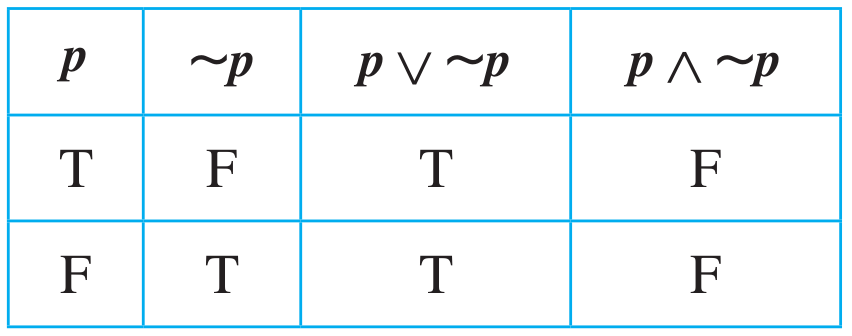
\includegraphics[scale=.25]{images/tautologi-kontradiksi}} 
	\end{figure} 
\end{frame}	

\begin{frame}{Contoh: Tautologi \& Kontradiksi}
	Jika $\mathbf{t}$ adalah tautologi dan $\mathbf{c}$ adalah kontradiksi, tunjukkan bahwa 
	\begin{equation*}
		p \wedge \mathbf{t} \equiv p
	\end{equation*}
	 dan 
	 \begin{equation*}
	 	p \wedge \mathbf{c} \equiv \mathbf{c}.
	 \end{equation*}
	
	\textbf{Jawab}:
	\begin{figure}[!ht]
	\centering
		\onslide<2->{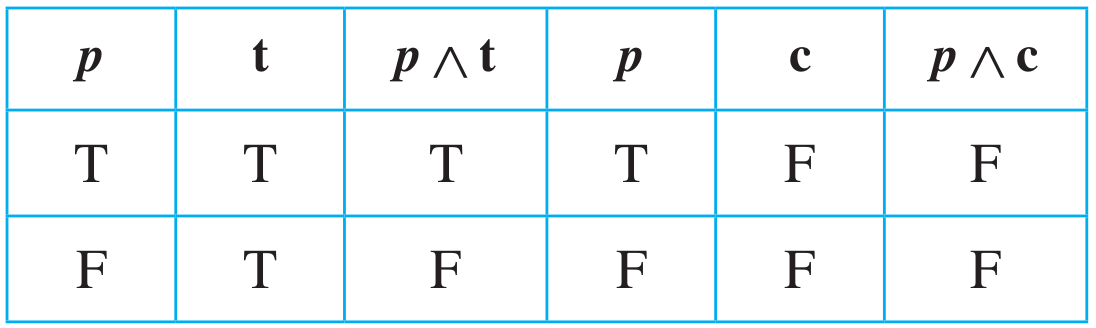
\includegraphics[scale=.25]{images/tautologi-kontradiksi-2}} 
	\end{figure} 
\end{frame}	

\section{Daftar Kesetaraan Logik}
\begin{frame}{Daftar Kesetaraan Logik}
	Berikut adalah \textbf{daftar kesetaraan logik} yang diambil dari \citet{epp2020discrete}:
	\begin{figure}[!ht]
		\centering
		\includegraphics<2->[scale=.2]{images/tabel-ekivalensi} 
	\end{figure}
\end{frame}	

\begin{frame}{Menyederhanakan Bentuk Statement}
	Tolong dicek kesetaraan logik berikut
	\begin{equation*}
		\mytilde ( \mytilde p \wedge q ) \wedge (p \vee q) \equiv p.
	\end{equation*}
	
	\onslide<2->{\textbf{Jawab}:} 
	\begin{align*}
		\onslide<3->{\mytilde ( \mytilde p \wedge q ) \wedge (p \vee q) &\equiv} \onslide<4->{(\mytilde (\mytilde p) \vee \mytilde q) \wedge (p \vee q)  && \text{\footnotesize by Hukum De Morgan}} \\
		\onslide<5->{&\equiv (p \vee \mytilde q) \wedge (p \vee q) && \text{\footnotesize by Hukum double negative} } \\
		\onslide<6->{&\equiv p \vee (\mytilde q \wedge q) && \text{\footnotesize by Hukum distributif} } \\ 
		\onslide<7->{&\equiv p \vee (q \wedge \mytilde q) && \text{\footnotesize by Hukum komutatif} } \\ 		
		\onslide<8->{&\equiv p \vee \mathbf{c} && \text{\footnotesize by Hukum negasi} } \\ 				
		\onslide<9->{&\equiv p && \text{\footnotesize by Hukum identitas} } 						
	\end{align*}	
\end{frame}

\section{Pernyataan Bersyarat}
\begin{frame}{Implikasi atau Jika-Maka}
	\onslide<2->{Diketahui $p$ dan $q$ adalah pernyataan.}\\
	\onslide<3->{Kalimat berbentuk "Jika $p$ maka $q$" diberi notasi "$p \rightarrow q$"}
	
	\onslide<4->{\textbf{Contoh I:}} 
	\begin{equation*}
	  	\onslide<5->{\underbrace{\text{Jika }4686 \text{ habis dibagi }6}_{\onslide<6->{\text{hipotesis}}}, \underbrace{\text{ maka }4686 \text{ habis dibagi }3.}_{\onslide<7->{\text{konklusi}}}}
	\end{equation*}

	\onslide<8->{\textbf{Contoh II:}} 
	\begin{equation*}
		\onslide<9->{\text{\textit{If you show up for work Monday morning, then you will get the job.}}}
	\end{equation*}
	\onslide<10->{Satu-satunya kombinasi yang menyatakan pernyataan di atas \textbf{false} terjadi ketika hipotesis \textbf{true} dan konklusi \textbf{false}} 
	\begin{equation*}
		\onslide<11->{\text{\textit{You do show up for work Monday morning and you do not get the job.}}}
	\end{equation*}
\end{frame}

\begin{frame}{Tabel Kebenaran untuk $p \rightarrow q$}
	Berikut tabel kebenaran untuk $p \rightarrow q$ yang diambil dari \citet{epp2020discrete}:

	\begin{figure}[!ht]
		\centering
		\includegraphics<2->[scale=.2]{images/jika-maka} 
	\end{figure}	
\end{frame}

\begin{frame}{Pernyataan Bersyarat yang \textit{Strange}}
	Pandang pernyataan
	\begin{equation*}
		\onslide<2->{\text{Jika }0 = 1 \text{ maka }1 = 2.} 
	\end{equation*}
	\onslide<2->{Apakah pernyataan di atas bernilai \textbf{true} atau \textbf{false}?} 
	
	\bigskip
	\onslide<3->{Pernyataan di atas bernilai \textbf{true}.}
\end{frame}

\begin{frame}{Representasi \textbf{Implikasi} sebagai \textbf{Atau}}
	Bentuk \textbf{Implikasi} dapat direpresentasikan dengan \textbf{Atau} sbb:
	\begin{equation*}
		\onslide*<2->{p \rightarrow q \equiv \mytilde p \vee q.} 
	\end{equation*}

	\onslide<3->{Tulis ulang pernyataan berikut dengan bentuk \textbf{Implikasi}.} 
	\begin{center}
		\onslide<3->{Either you get to work on time or you are fired.} 
	\end{center}

	\onslide<4->{\textbf{Jawab}:}
	\begin{center}
		\onslide<4->{If you do not get to work on time, then you are fired.} 
	\end{center}
\end{frame}

\begin{frame}{Negasi dari Pernyataan Bersyarat}
\begin{equation*}
	\mytilde (p \rightarrow q) \equiv p \wedge \mytilde q
\end{equation*}

\onslide<2->{Caranya:}
\begin{align*}
	\onslide<2->{\mytilde ( p \rightarrow q ) &\equiv}  \onslide<3->{\mytilde ( \mytilde p \wedge q ) \\} 
	                             \onslide<4->{&\equiv \mytilde ( \mytilde p ) \wedge (\mytilde q) && \text{by Hukum De Morgan} \\} 
	                             \onslide<5->{&\equiv p \wedge \mytilde q && \text{by hukum double negative}} 
\end{align*}

\onslide<6->{Tuliskan \textbf{negasi} dari pernyataan-pernyataan berikut!}
\begin{itemize}
	\item<7-> If my car is in the repair shop, then I cannot get to class.
	\item<8-> If Sara lives in Athens, then she lives in Greece. 
\end{itemize}

\onslide<9->{\textbf{Jawab:}} 
\begin{itemize}
	\item<10->{My car is in the repair shop and I can get to class.}
	\item<11->{Sara lives in Athens and she does not live in Greece.} 
\end{itemize}
\end{frame}

\begin{frame}{Kontrapositif dari Pernyataan Bersyarat}
	\begin{block}<2->{Definisi}
		Kontrapositif dari pernyataan bersyarat yang berbentuk "Jika $p$ maka $q$" adalah
		\begin{equation*}
			\text{If }\mytilde q \text{ then } \mytilde p.
		\end{equation*}
		Dengan simbol, kontrapositif dari $p \rightarrow q$ adalah $\mytilde q \rightarrow \mytilde p$.
	\end{block}

	\onslide<3->{Fakta menyatakan bahwa} 
	
	\bigskip
	\onslide<4->{\textit{Pernyataan bersyarat memiliki \textbf{kesetaraan logik} dengan kontrapositif-nya}}
\end{frame}

\begin{frame}{Biimplikasi}
	\begin{block}<2->{Definisi}
		Diberikan dua pernyataan $p$ dan $q$, \textbf{biimplikasi dari} $\bm{p}$ \textbf{dan} $\bm{q}$ adalah "$p$ jika dan hanya jika $q$" dan diberi notasi $p \leftrightarrow q$. 
	\end{block}
	\onslide<3->{Tabel kebenaran \textbf{biimplikasi} adalah sebagai berikut \citep{epp2020discrete}:} 
	\begin{figure}[!ht]
		\centering
		\includegraphics<4->[scale=.25]{images/tabel-biimplikasi}
	\end{figure}
\end{frame}

\section{Argumen yang Valid dan Invalid}
\begin{frame}{Argumen}
	\onslide<2->{\textbf{Argumen} adalah barisan dari pernyataan-pernyataan yang diakhiri dengan kesimpulan.} 
	
	\bigskip
	\onslide<3->{Contoh:} 
	\begin{align*}
		\onslide<4->{& \text{If Socrates is a man, then Socrates is mortal.} \\}        
        \onslide<5->{& \text{Socrates is a man.} \\}		        
	    \onslide<6->{\therefore \text{ }& \text{Socrates is mortal.}} 
	\end{align*}
	\onslide<7->{mempunyai bentuk abstrak}
	\begin{align*}
		\onslide<8->{& \text{Jika }p \text{ maka }q \\}        
		\onslide<9->{& p \\}		        
		\onslide<10->{\therefore \text{ }& q} 
	\end{align*}
\end{frame}

\begin{frame}{Argumen yang Valid}
	Diberikan suatu argumen sebagai berikut:
	\begin{align*}
	\onslide<2->{& \text{Jika }p \text{ maka }q \\}        
	\onslide<2->{& p \\}		        
	\onslide<2->{\therefore \text{ }& q} 
	\end{align*}
	
	\onslide<3->{Tabel kebenaran dari argumen di atas adalah:}
	\onslide<4->{
	\begin{table}[!ht]
		\centering
		\begin{tabular}{|c|c|c|c|c|}
			\hline
			$\bm{p}$ & $\bm{q}$ & $\bm{p \rightarrow q}$ & $\bm{p}$ & $\bm{q}$ \\
			\hline
			T & T & T & T & T \\
			\hline
			T & F & F & T & F \\
			\hline
			F & T & T & F & T \\
			\hline
			F & F & T & F & F \\
			\hline  
		\end{tabular}
	\end{table}}
\end{frame}

\begin{frame}{Argumen yang Tidak Valid}
	Diberikan suatu argumen sebagai berikut:
	\begin{align*} 
		\onslide<2->{& p \rightarrow q \vee \mytilde r \\}        
		\onslide<2->{& q \rightarrow p \wedge r \\}		        
		\onslide<2->{\therefore \text{ }& p \rightarrow r } 
	\end{align*}
	
	\onslide<3->{Tabel kebenaran dari argumen di atas adalah \citep{epp2020discrete}:}
	\begin{figure}[!ht]
		\centering
		\includegraphics<4->[scale=.175]{images/contoh-tidak-valid}
	\end{figure}	

\end{frame}

\section{Modus Ponens \& Modus Tollens}
\begin{frame}{Modus Ponens}
	\begin{itemize}
		\item<2-> Suatu argumen yang terdiri dari \textbf{dua premis} dan \textbf{satu kesimpulan} disebut \textbf{silogisme}.
		\item<3-> Premis pertama disebut \textbf{premis mayor}.
		\item<4-> Premis kedua disebut \textbf{premis minor}.
		\item<5-> Bentuk silogisme paling terkenal di dalam logika disebut \textbf{modus ponens}.
	\end{itemize}		
	\onslide<6->{Bentuk modus ponens:} 
	\onslide<7->{
	\begin{align*}
		          & \text{Jika }p \text{ maka }q \\
		          & p	 \\
	  \therefore  & q	
	\end{align*}}	
	\onslide<8->{\textbf{Contoh:}}
	\begin{align*}
		\onslide<9->{& \text{Jika jumlah digit dari }371487 \text{ habis dibagi }3, \text{ maka}}  \\
		\onslide<9->{& 371487 \text{ habis dibagi }3. }\\
		\onslide<10->{& \text{Jumlah digit dari }371487 \text{ habis dibagi }3.} \\                 
    \onslide<11->{\therefore \text{ }  & 371487 \text{ habis dibagi }3.	}	
	\end{align*}			
\end{frame}

\begin{frame}{Modus Tollens}
	\onslide<2->{Bentuk silogisme lain adalah \textbf{modus tollens} yang memiliki bentuk:}
	\onslide<3->{
	\begin{align*}
		          & \text{Jika }p \text{ maka }q \\
		          & \mytilde q \\
	 \therefore	  & \mytilde p
	\end{align*}}
	\onslide<4->{\textbf{Contoh:}}
\begin{align*}
	\onslide<5->{& \text{Jika Zeus adalah manusia, maka Zeus makhluk fana}}  \\
	\onslide<6->{& \text{Zeus bukan makhluk fana}}\\
	\onslide<7->{\therefore \text{ }  & \text{Zeus bukan manusia}}	
\end{align*}			
\end{frame}

\section{Soal-Soal KSNK 2020}
\begin{frame}{KSNK 2020: Soal Logika I}
	\begin{figure}[!ht]
		\centering
		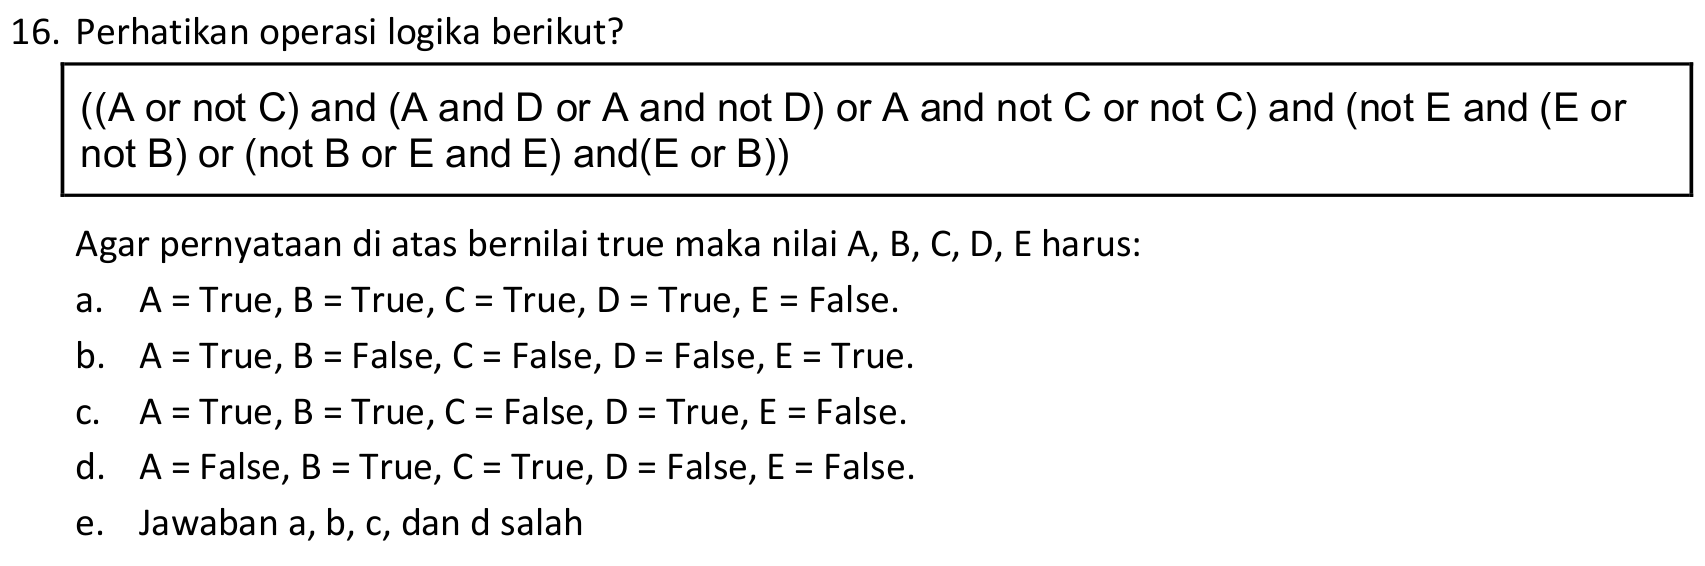
\includegraphics[scale=.19]{images/soal-ksnk-2020-no-16-logika}
	\end{figure}
\end{frame}

\begin{frame}{KSNK 2020: Soal Logika I}
	\begin{figure}[!ht]
		\centering
		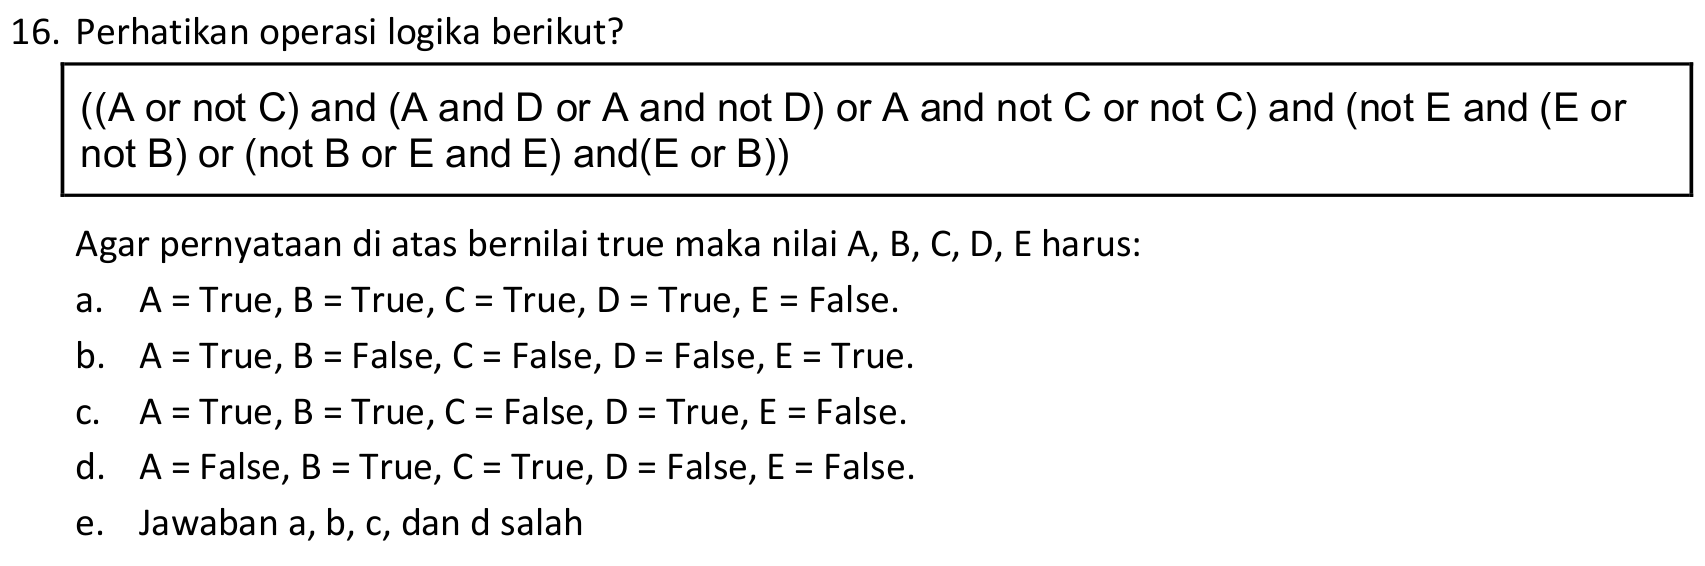
\includegraphics[scale=.19]{images/soal-ksnk-2020-no-16-logika}
	\end{figure}
\end{frame}

\begin{frame}{KSNK 2020: Solusi Logika I}
	\begin{center}
		Silakan Teman-teman untuk mencobanya.
	\end{center}
\end{frame}

\begin{frame}{KSNK 2020: Soal Logika II}
	\begin{figure}[!ht]
		\centering
		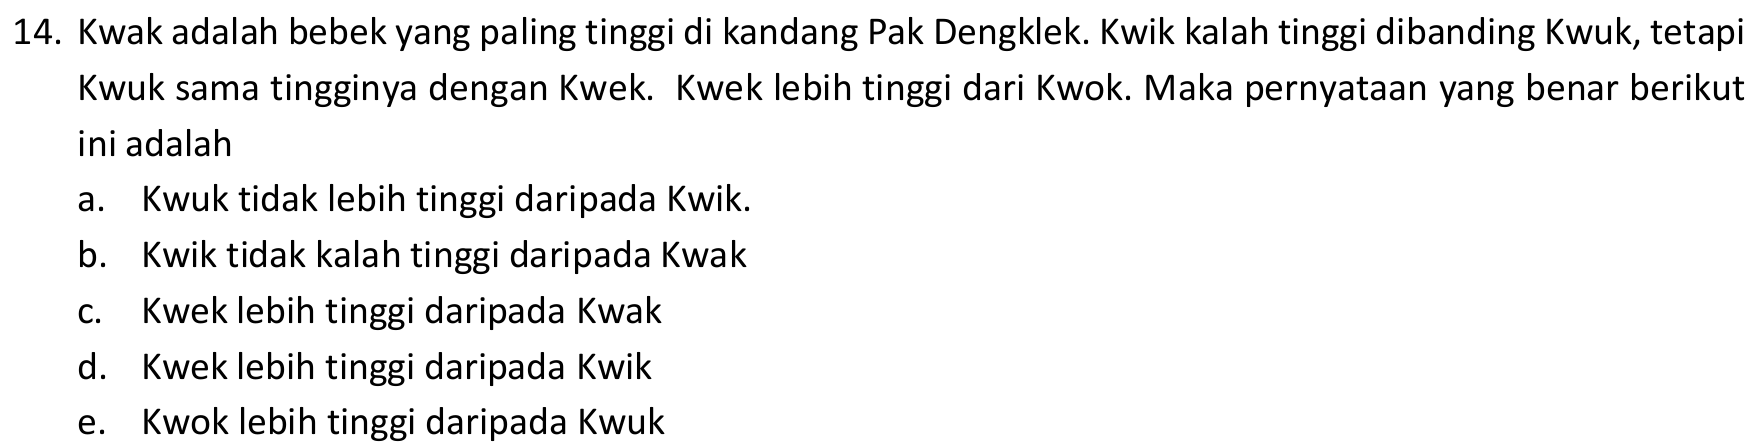
\includegraphics[scale=.19]{images/soal-ksnk-2020-no-14-logika}
	\end{figure}
\end{frame}

\begin{frame}{KSNK 2020: Solusi Logika II}
	\begin{center}
		Silakan Teman-teman untuk mencobanya.
	\end{center}	
\end{frame}

\begin{frame}{KSNK 2020: Soal Logika III (1/2)}
Angga, Bandi dan Cinta diinterogasi oleh polisi atas pembunuhan dari Duduy. Bukti-bukti pada tempat kejadian perkara (TKP) menunjukkan bahwa \textit{mungkin seorang pengacara terlibat pada perkara pembunuhan}. Mereka, salah satunya adalah pembunuh, membuat dua buah pernyataan sebagai berikut.
\begin{itemize}
	\item Angga memberi pernyataan:
		\begin{itemize}
			\item Saya bukan pengacara
			\item Saya tak terlibat pembunuhan Duduy
		\end{itemize}
	\item Bandi memberi pernyataan:
		\begin{itemize}
			\item Saya memang seorang pengacara
			\item Tetapi saya tak terlibat pembunuhan Duduy
		\end{itemize}
	\item Cinta memberikan pernyataan
		\begin{itemize}
			\item Saya bukan pengacara
			\item Seorang pengacara yang membunuh Duduy
		\end{itemize}
\end{itemize}
\end{frame}

\begin{frame}{KSNK 2020: Soal Logika III (2/2)}
	Pada pemeriksaan polisi ditemukan bahwa hanya dua dari pernyataan di atas yang benar dan ternyata hanya satu dari ketiga orang itu yang bukan pengacara.

	\bigskip
	Siapakah yang membunuh Duduy?
	\begin{enumerate}
		\item Angga
		\item Bandi
		\item Cinta
		\item Angga dan Bandi bersama-sama
		\item Jawaban 1, 2, 3, dan 4 salah.
	\end{enumerate}
\end{frame}

\begin{frame}{KSNK 2020: Solusi Logika III}
	\begin{center}
		Silakan Teman-teman untuk mencobanya.
	\end{center}	
\end{frame}












	
	
	
	
	
	
	
	
	
	
	
	
	
	%%%% predictive distribution
	
	
	% \begin{frame}
		%   \frametitle{Some other one parameter models}
		
		%   \begin{itemize}
			%   \item Poisson
			%   \item Exponential
			%   \item Cauchy
			%   \end{itemize}
		
		% \end{frame}
	
	\section<presentation>*{\appendixname}
	\subsection<presentation>*{For Further Reading}
	
	\begin{frame}[allowframebreaks]
		\frametitle<presentation>{Daftar Pustaka}
		{\footnotesize
			%    \bibliographystyle{apalike}
			\bibliography{references}
		}    
	\end{frame}
	
\end{document}

%%% Local Variables: 
%%% TeX-PDF-mode: t
%%% TeX-master: t
%%% End: 
